\section{Experiments}
\label{sec:experiments}

\subsection{Questions and Reporting Policy}
We organize the study around six research questions:
\begin{itemize}
    \item \textbf{RQ1:} Are damage probabilities calibrated enough for action selection?
    \item \textbf{RQ2:} Does the policy identify when reinspection is useful better than no, random, fixed, and heuristic controls?
    \item \textbf{RQ3:} Does reinspection improve damage judgment on evidence-bearing episodes?
    \item \textbf{RQ4:} What judgment or uncertainty gain is obtained per extra action and meter flown?
    \item \textbf{RQ5:} How robust are calibration and decisions on held-out events and degraded observations?
    \item \textbf{RQ6:} How does active reinspection affect navigation \(\SR\), \(\NE\), \(\SPL\), and path length?
\end{itemize}
We report all available evidence for these questions, including negative and compromised results.
Navigation gains are never inferred from perception-only metrics, and \(\semSR\) is never treated as strict success.

\subsection{RQ6: Navigation Ablation Remains Low and Inconclusive}
\begin{table}[t]
\centering
\caption{Strict E1 navigation under the event-disjoint U-Net proposer
(40 tasks, three paired seeds, hybrid grounding). Every configuration has
zero strict success.}
\label{tab:navigation}
\resizebox{\columnwidth}{!}{
% Auto-generated by scripts/benchmarks/export_paper_assets.py
\begin{tabular}{lrrrrrr}
\toprule
Method & SR (\%) $\uparrow$ & semSR (\%) $\uparrow$ & NE $\downarrow$ & semNE $\downarrow$ & SPL $\uparrow$ & Steps $\downarrow$ \\
\midrule
B0 & 7.5 & 12.5 & 150.0 & 136.4 & 0.072 & 3.27 \\
B1 & 7.5 & 12.5 & 225.7 & 193.3 & 0.068 & 4.75 \\
B2 & 2.5 & 15.0 & 230.4 & 190.0 & 0.025 & 5.58 \\
B3 & 2.5 & 7.5 & 300.6 & 261.2 & 0.025 & 5.50 \\
\bottomrule
\end{tabular}
}
\end{table}


\tabref{tab:navigation} reports the historical 40-instruction, single-repeat E1 run.
Strict success is low for every configuration.
Adding the hierarchical planner leaves \(\SR\) unchanged at 0.075 while increasing navigation error.
Adding reinspection or memory does not improve strict success.
The slight semantic-success difference for reinspection is not a substitute for strict target arrival.
With this sample size, the navigation differences are not statistically significant.
These results establish a difficult benchmark and expose grounding failures; they do not establish that the supporting stack improves navigation.
The strict evidence-rich rerun with hybrid grounding, three paired seeds, and the event-disjoint perception stack is \pending.

\subsection{RQ1: Calibration Helps In-Domain Confidence, Not Uniformly}
\begin{table}[t]
\centering
\caption{Strict event-disjoint temperature scaling for the concatenation
baseline. Accuracy is unchanged; test ECE improves, while holdout ECE
worsens under the validation-fitted temperature.}
\label{tab:calibration}
\resizebox{\columnwidth}{!}{
% Auto-generated by scripts/benchmarks/export_paper_assets.py
\begin{tabular}{llrrrr}
\toprule
Split & Calibration & Acc. $\uparrow$ & ECE $\downarrow$ & Brier $\downarrow$ & NLL $\downarrow$ \\
\midrule
Test & Uncalibrated & 0.765 & 0.095 & 0.398 & 0.813 \\
Test & Temperature scaled & 0.765 & 0.037 & 0.387 & 0.778 \\
Holdout & Uncalibrated & 0.803 & 0.046 & 0.340 & 0.704 \\
Holdout & Temperature scaled & 0.803 & 0.084 & 0.348 & 0.713 \\
\bottomrule
\end{tabular}
}
\end{table}


Under the frozen event-disjoint split, temperature scaling changes test ECE from 0.095 to 0.037 while leaving accuracy unchanged at 0.765 (\tabref{tab:calibration}).
On the held-out events, the same validation-fitted temperature increases ECE from 0.046 to 0.084.
Brier score and NLL improve on test and worsen slightly on holdout.
Thus calibrated probabilities are useful for the in-domain test partition, but a single scalar temperature is not a sufficient robustness guarantee for held-out disasters.

\begin{figure}[t]
  \centering
  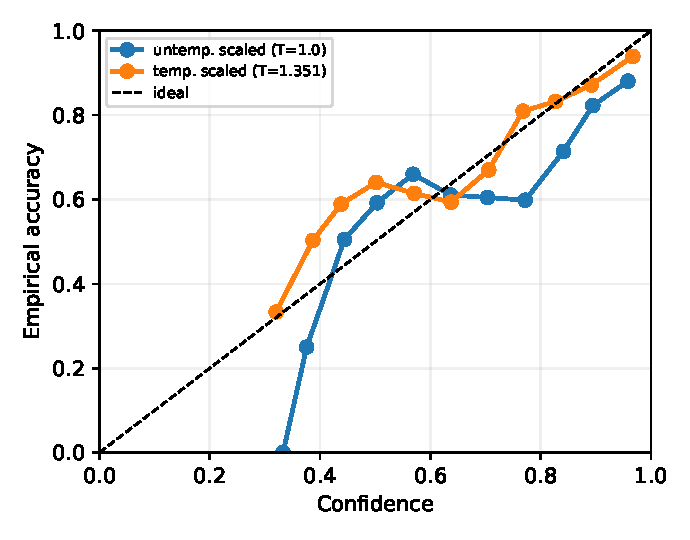
\includegraphics[width=\columnwidth]{generated/calibration_reliability.pdf}
  \caption{Strict event-disjoint test-set reliability before and after
  scalar temperature scaling fitted on validation.}
  \label{fig:reliability}
\end{figure}

\subsection{RQ5: Strict Difference Attention Does Not Repeat the Old Holdout Gain}
\begin{table}[t]
\centering
\caption{Strict event-disjoint temporal-fusion comparison after temperature
scaling. Accuracy is nearly identical; neither fusion dominates every
calibration metric.}
\label{tab:difference_attention}
\resizebox{\columnwidth}{!}{
% Auto-generated by scripts/benchmarks/export_paper_assets.py
\begin{tabular}{llrrrr}
\toprule
Split & Fusion & Acc. $\uparrow$ & ECE $\downarrow$ & Brier $\downarrow$ & NLL $\downarrow$ \\
\midrule
Test & Concatenation & 0.765 & 0.037 & 0.387 & 0.778 \\
Test & Difference attention & 0.765 & 0.035 & 0.379 & 0.787 \\
Holdout & Concatenation & 0.803 & 0.084 & 0.348 & 0.713 \\
Holdout & Difference attention & 0.803 & 0.111 & 0.362 & 0.744 \\
\bottomrule
\end{tabular}
}
\end{table}


After event-disjoint retraining, concatenation and difference attention reach nearly identical accuracy on test and holdout (\tabref{tab:difference_attention}).
Calibrated test ECE slightly favors difference attention, while calibrated holdout ECE favors concatenation.
The earlier historical observation that difference attention substantially raised holdout accuracy therefore does not survive the strict protocol.
\begin{table}[t]
\centering
\caption{Frozen event-disjoint split used by the strict perception and
calibration protocol. No disaster event appears in more than one partition.}
\label{tab:event-split}
\resizebox{\columnwidth}{!}{
% Auto-generated by scripts/benchmarks/export_paper_assets.py
\begin{tabular}{lcp{5.2cm}}
\toprule
Split & \#Events & Event names \\
\midrule
train & 12 & 12 remaining events (appendix) \\
val & 2 & hurricane-harvey, mexico-earthquake \\
test & 2 & hurricane-michael, palu-tsunami \\
holdout & 3 & moore-tornado, nepal-flooding, pinery-bushfire \\
\bottomrule
\end{tabular}
}
\end{table}

\tabref{tab:event-split} records the frozen partition.
\begin{table}[t]
\centering
\caption{Strict event-disjoint YOLOv8s detector metrics used by hybrid
grounding. Low recall remains a localization bottleneck.}
\label{tab:yolo-metrics}
\resizebox{\columnwidth}{!}{
% Auto-generated by scripts/benchmarks/export_paper_assets.py
\begin{tabular}{lrrrr}
\toprule
Split & P $\uparrow$ & R $\uparrow$ & mAP@0.5 $\uparrow$ & mAP@0.5:0.95 $\uparrow$ \\
\midrule
val & 0.148 & 0.094 & 0.042 & 0.017 \\
test & 0.257 & 0.237 & 0.144 & 0.061 \\
holdout & 0.403 & 0.203 & 0.175 & 0.089 \\
\bottomrule
\end{tabular}
}
\end{table}

The detector used for hybrid grounding remains weak under the same split (\tabref{tab:yolo-metrics}); low recall is a localization bottleneck for language-conditioned targeting.

\subsection{RQ2--RQ4: Active Reinspection Is Currently Underpowered}
The available E11 study evaluates six policies on 40 episodes.
Pairwise strict-SR differences are non-significant (\(p\geq0.49\)).
Only one episode contains detected damage evidence and activates genuine reinspection; the other 39 remain at \texttt{risk\_level=none}.
Although that single episode shows different uncertainty changes across policies, \(n=1\) cannot support a positive conclusion for when to reinspect, judgment gain, or cost-normalized utility.
The current evidence therefore demonstrates execution and logging, not effectiveness.

\begin{figure}[t]
  \centering
  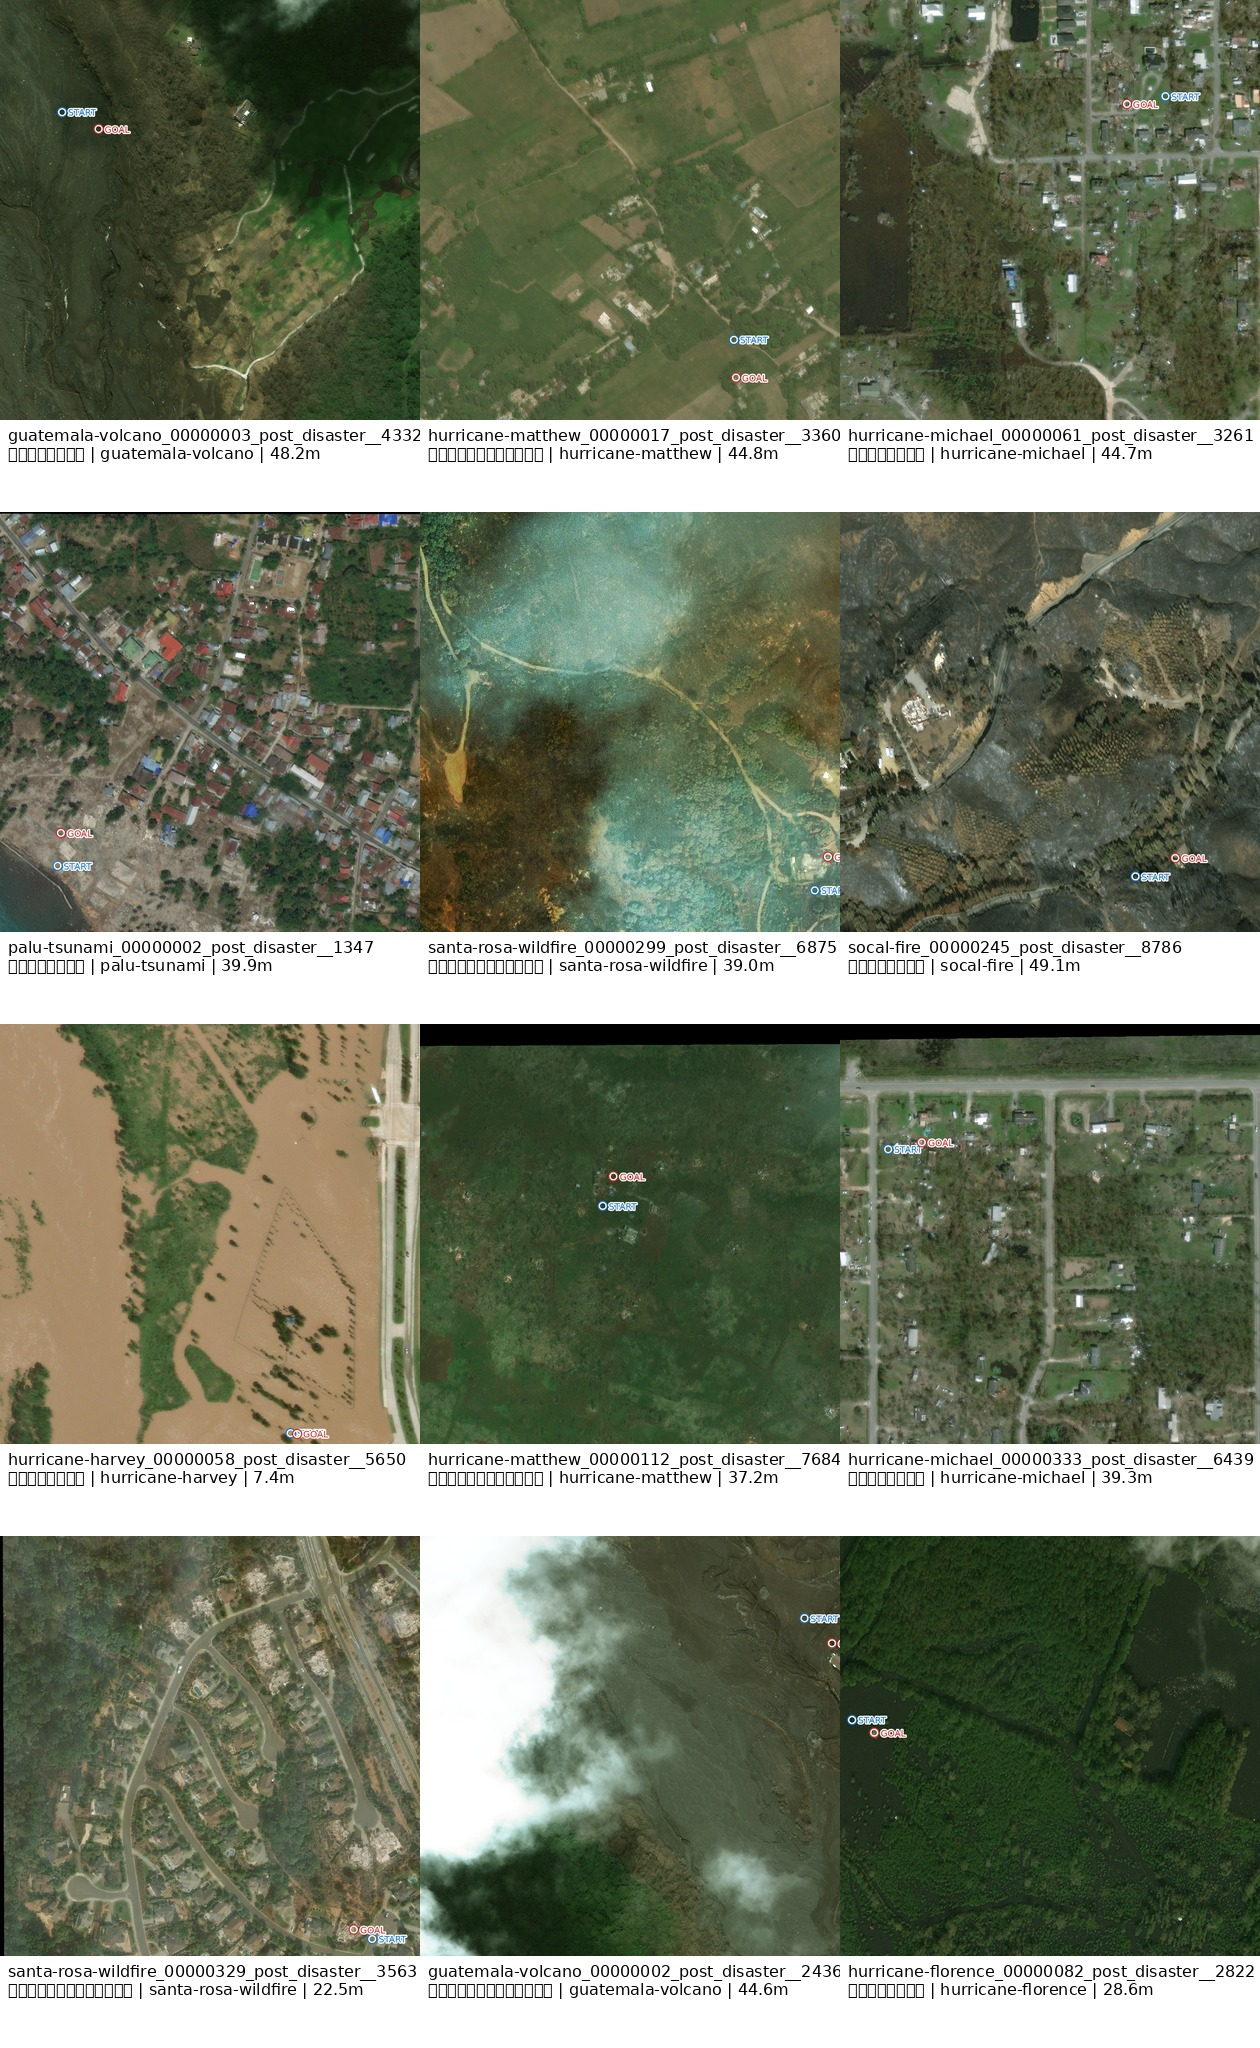
\includegraphics[width=\columnwidth]{generated/review_sheets/review_01.jpg}
  \caption{Contact-sheet audit for the evidence-rich reinspection subset.
  Starts are outside the 25\,m success radius and inside the default
  observation radius; approval is geometry-checked and visually reviewed.
  Strict policy comparison on this set is \pending.}
  \label{fig:evidence-rich}
\end{figure}

An evidence-rich 40-task subset with starts outside the success radius has been frozen for the strict rerun (\figref{fig:evidence-rich}); its results are \pending.

\subsection{Pre-Registered Strict Evaluation}
Event-disjoint manifests, perception checkpoints, and calibration fits are now frozen.
Remaining work is the paired navigation and reinspection suite with hybrid grounding, three seeds, bootstrap confidence intervals, Wilcoxon or paired permutation tests, and Holm correction over the six-policy family.
No positive claim will be made if trigger coverage is too low for the pre-specified analysis.
Appendix~\ref{app:protocol} records the frozen hypotheses and denominators.
